\documentclass[../../main.tex]{subfiles}

\begin{document}

\subsection{Motivation}

It is considered a problem of constructing a phase trajectory of a video file using tensor-based singular spectrum analysis method. Usually, phase trajectory of a time series is constructed using SSA method that is applied to a matrix with two indices \cite{golyandina, usmanova}. In this work it is proposed to apply tensor-based SSA method that constructs a trajectory matrix that has 3 indices, then apply HOSVD method for extracting principal components.

\subsection{Problem statement}

Given a sequence of images that composes a gray-scale video. Let us consider this as a time series system. Each time series is a sequence of a particular pixel brightness:

$$F^{(k)} = (f_j^{(k)})_{j=0}^{N-1}, \quad k = 1, \dots, hw,$$

\noindent
where $h$ is the video height, $w$ is the video width, $hw$ is a number of signals with length $N$.

The purpose is to construct a phase trajectory of the time series system and make a forecast $\hat{\mathbf{X}}^\prime$ using tensor-based SSA method and HOSVD.

\subsection{Problem solution}

It is proposed to solve a problem with tensor-based singular spectrum analysis and make a forecast using HOSVD.

\textbf{1st step: Embedding}

Let $L$ be a window length, $1 < L < N$. The embedding procedure forms $K = N-L+1$ lagged vectors for every time series:

$$X_l^{(k)} = (f_{l-1}^{(k)}, \dots, f_{l+L-2}^{(k)})^\top.$$

The trajectory matrix of the time series system $F^{(1)}, \dots, F^{(hw)}$ is a tensor that has a form

$$\hat{\mathbf{X}} = (\mathbf{X}^{(1)}, \dots, \mathbf{X}^{(hw)}),$$

\noindent
where $\mathbf{X}^{(k)} = (X_l^{(k)})_{l=0}^{K}$.

\textbf{2nd step: HOSVD}

Truncated HOSVD is performed:

$$\hat{\mathbf{X}} = \mathbf{S} \times_1 U_1 \times_2 U_2 \times_3 U_3,$$

\noindent
where $\mathbf{S}$ is a core tensor, $U_1, U_2, U_3$ are matrices with unitary columns containing a basis of the left singular vectors corresponding to the nonzero singular values of the standard factor-$k$ flattening $X_{(k)}$ of $X$ for $k = 1, 2, 3$.

The HOSVD of $\hat{\mathbf{X}}$ can be represent as

$$\hat{\mathbf{X}} = \hat{\mathbf{X}}_1 + \dots + \hat{\mathbf{X}}_d,$$

\noindent
where $\hat{\mathbf{X}}_i$ has rank equal to 1.

\textbf{3rd step: Grouping}

The grouping procedure partitions the
set of indices $\{1, \dots, d\}$ into $m$ disjoint subsets $I_1, \dots, I_m$. Let $I = {i_1, \dots, i_p}$. Then the resultant matrix $\hat{\mathbf{X}}$ corresponding to the group $I$ is defined as $\hat{\mathbf{X}}_I = \hat{\mathbf{X}}_{i_1} + \dots + \hat{\mathbf{X}}_{i_p}$. Thus, we have the grouped decomposition:

$$\hat{\mathbf{X}} = \hat{\mathbf{X}}_{I_1} + \dots + \hat{\mathbf{X}}_{I_m}.$$

\textbf{4th step: Diagonal averaging}

The last step is in a sense opposite to the first step and transforms each matrix of the grouped decomposition into a system of new (reconstructed) series of length $N$ by hankelization-like procedure.

\subsection{Code analysis}

Code for HOSVD decomposition was taken from GitHub repository\footnote{https://github.com/hottbox/hottbox}. Code of the computational experiment can be found in the repository\footnote{https://github.com/gorpinich-m/Math-methods-of-forecasting}.

\subsection{Experiment}

\begin{figure}[h!]
\centering
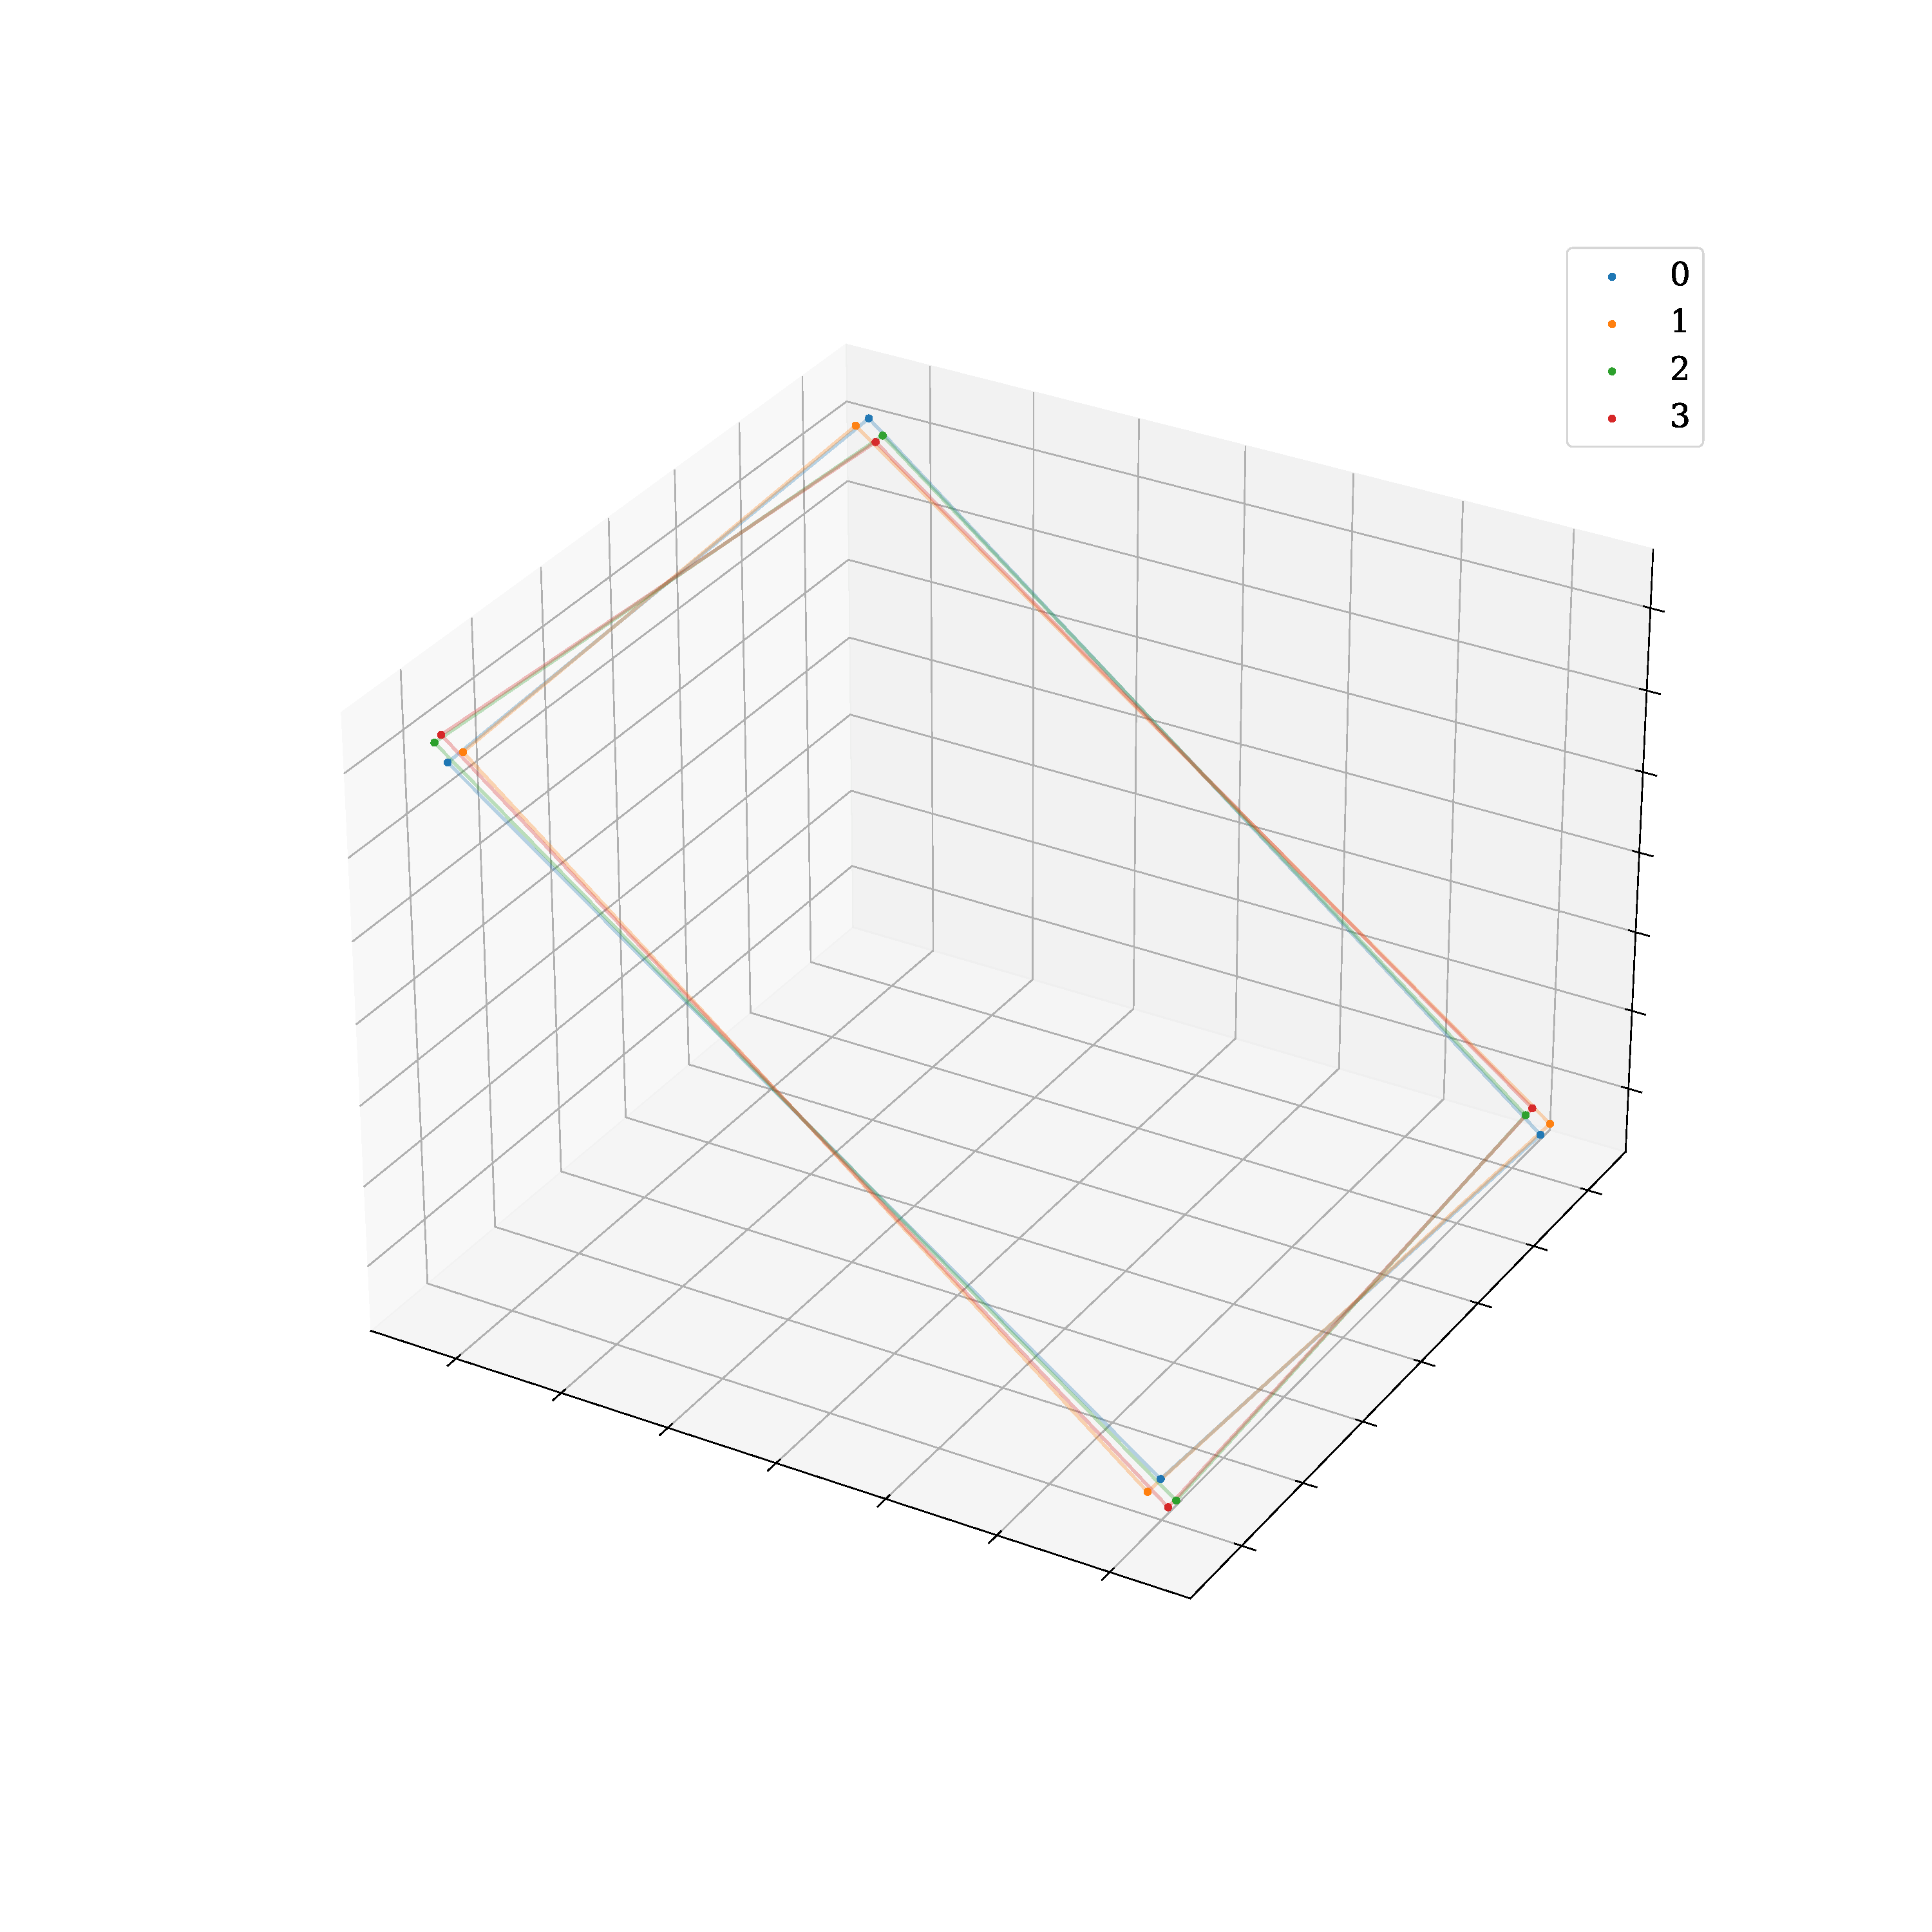
\includegraphics[width=0.8\textwidth]{sections/gorpinich/trajectories_base.pdf}
\caption{Some description}
\label{fig:1}
\end{figure}

Fig. \ref{fig:1} plots phase trajectories of 4 pixels of the basic video.

\begin{figure}[h!]
\centering
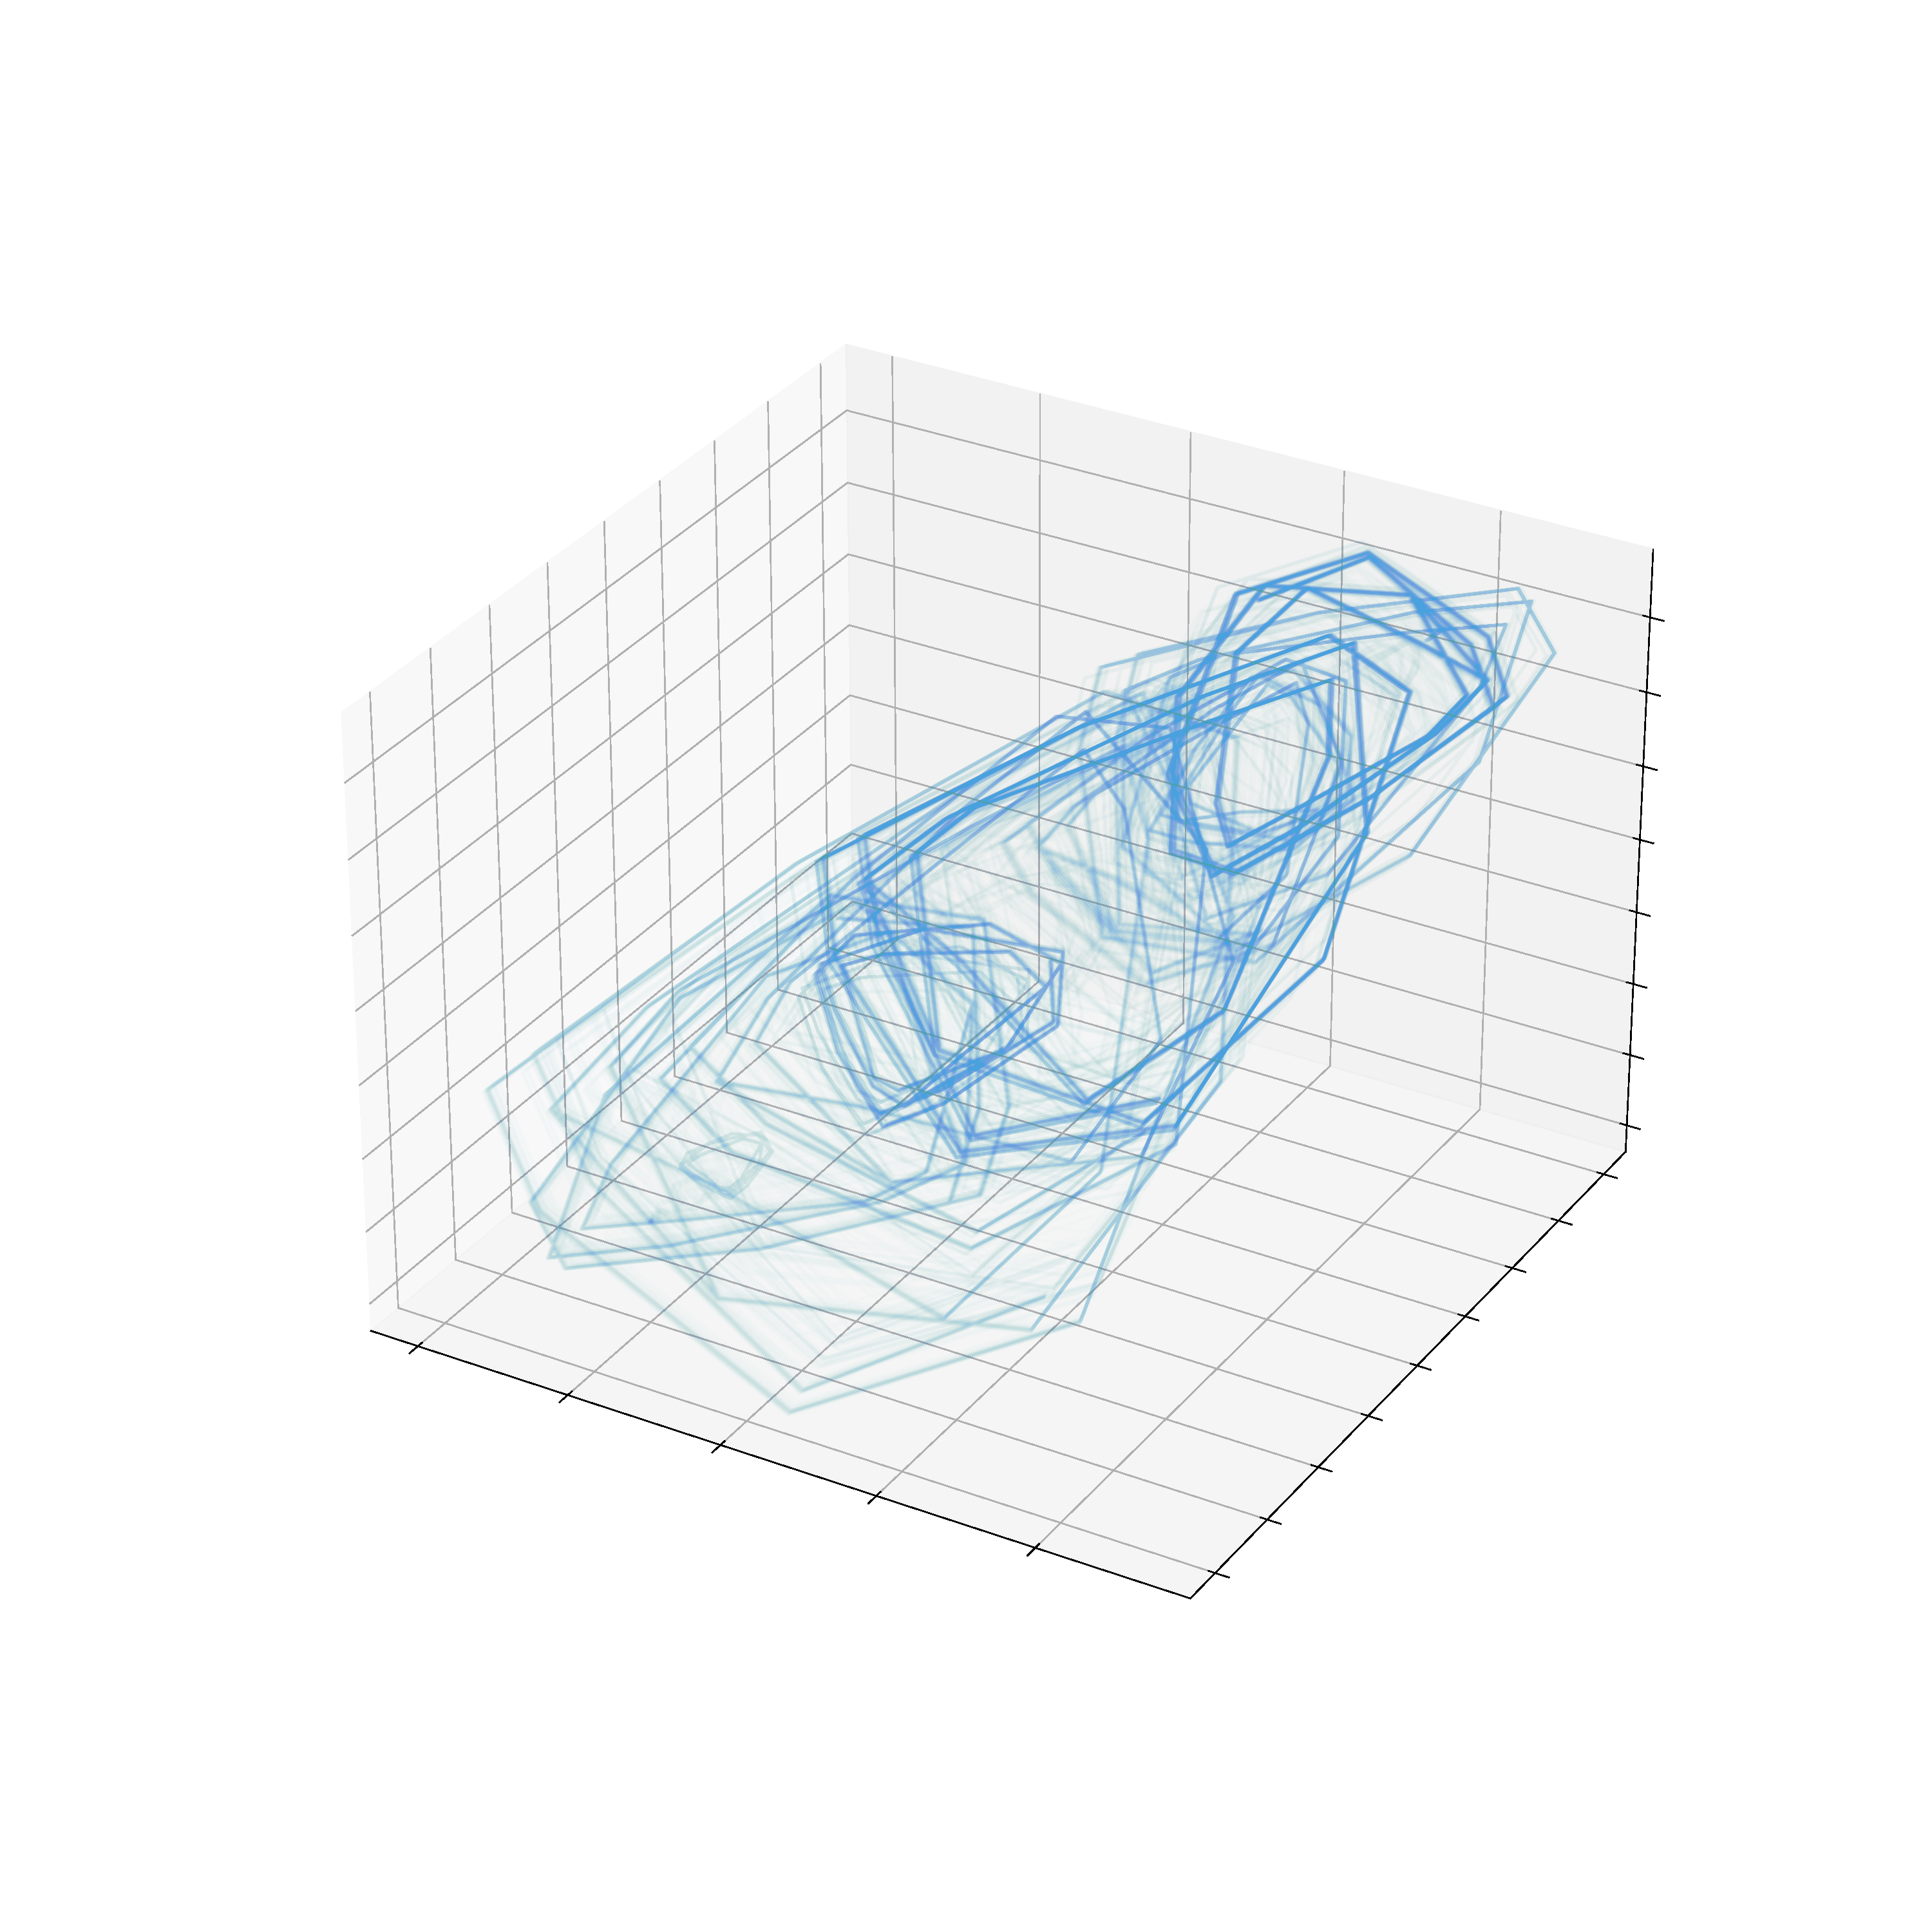
\includegraphics[width=0.8\textwidth]{sections/gorpinich/mario_trajectory.pdf}
\caption{Some description}
\label{fig:2}
\end{figure}

Fig. \ref{fig:1} plots phase trajectories of 1000 pixels of the video.

\begin{figure}[h!]
\centering
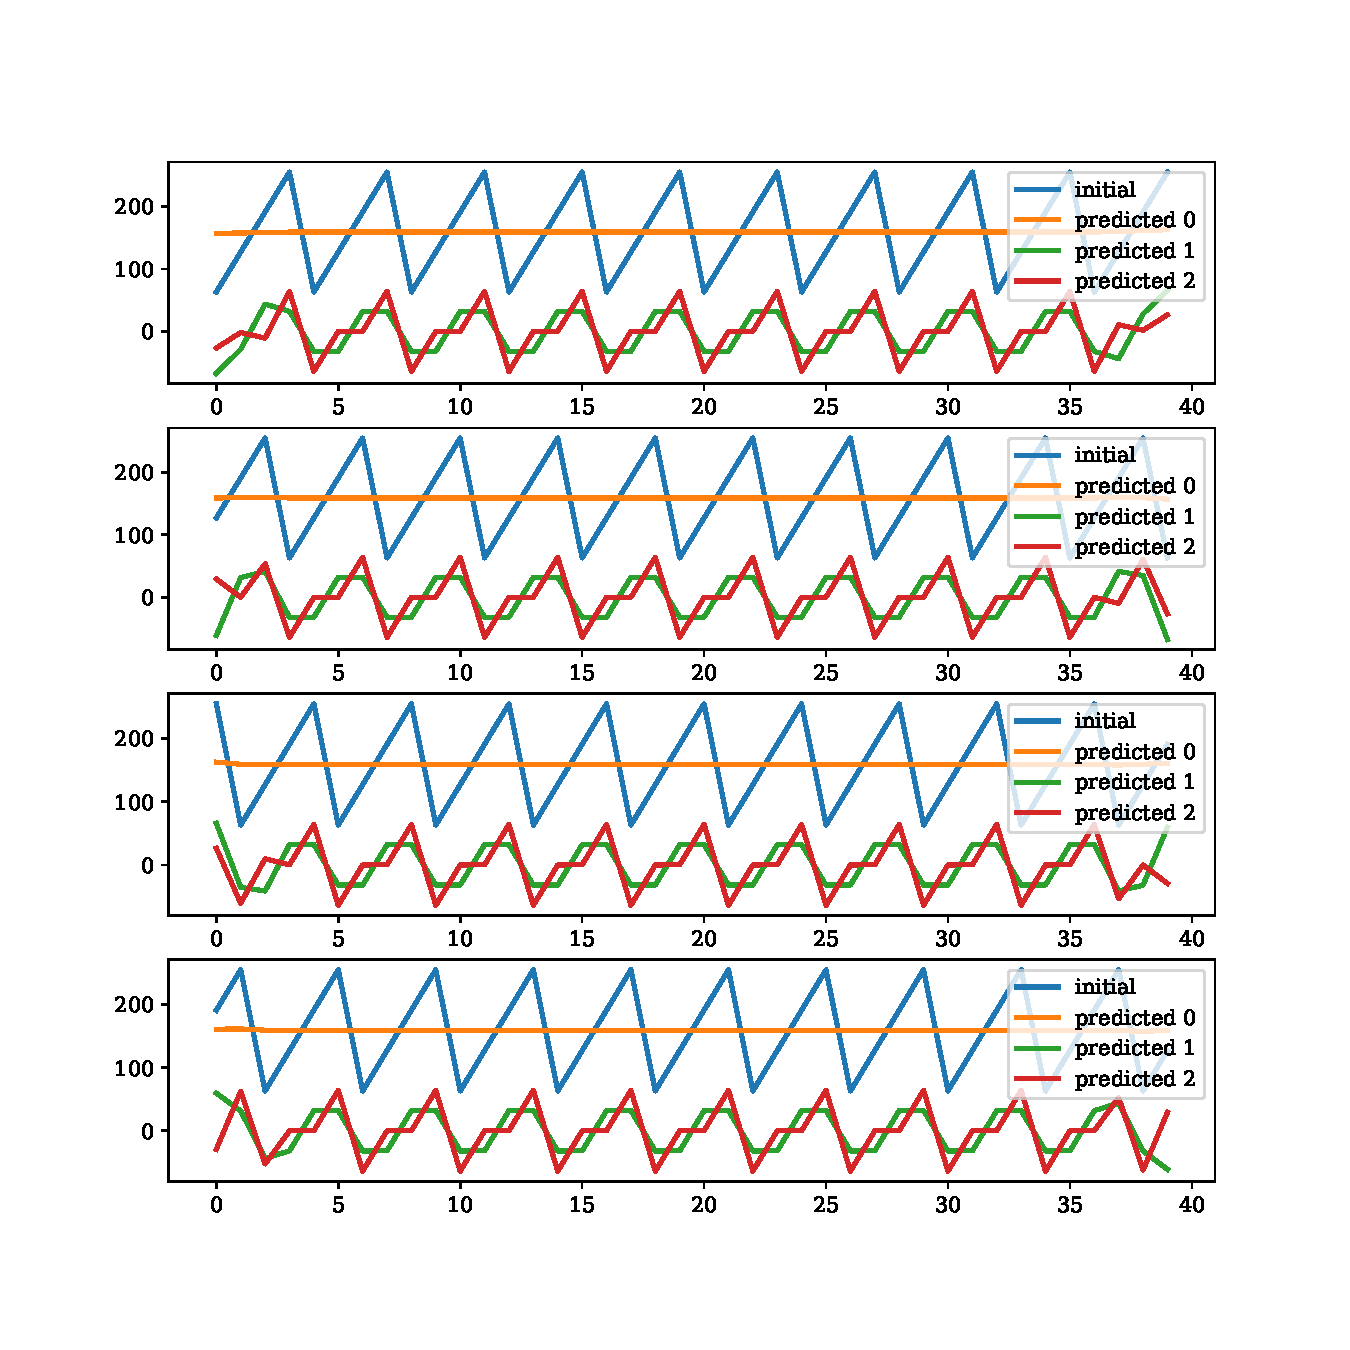
\includegraphics[width=0.6\textwidth]{sections/gorpinich/ssa_base.pdf}
\caption{Some description}
\label{fig:3}
\end{figure}

Fig. \ref{fig:3} plots SSA decomposition of the basic video. We can see that the first component is a trend and other 2 components depict periodicity ans seasonality.

\begin{figure}[h!]
\centering
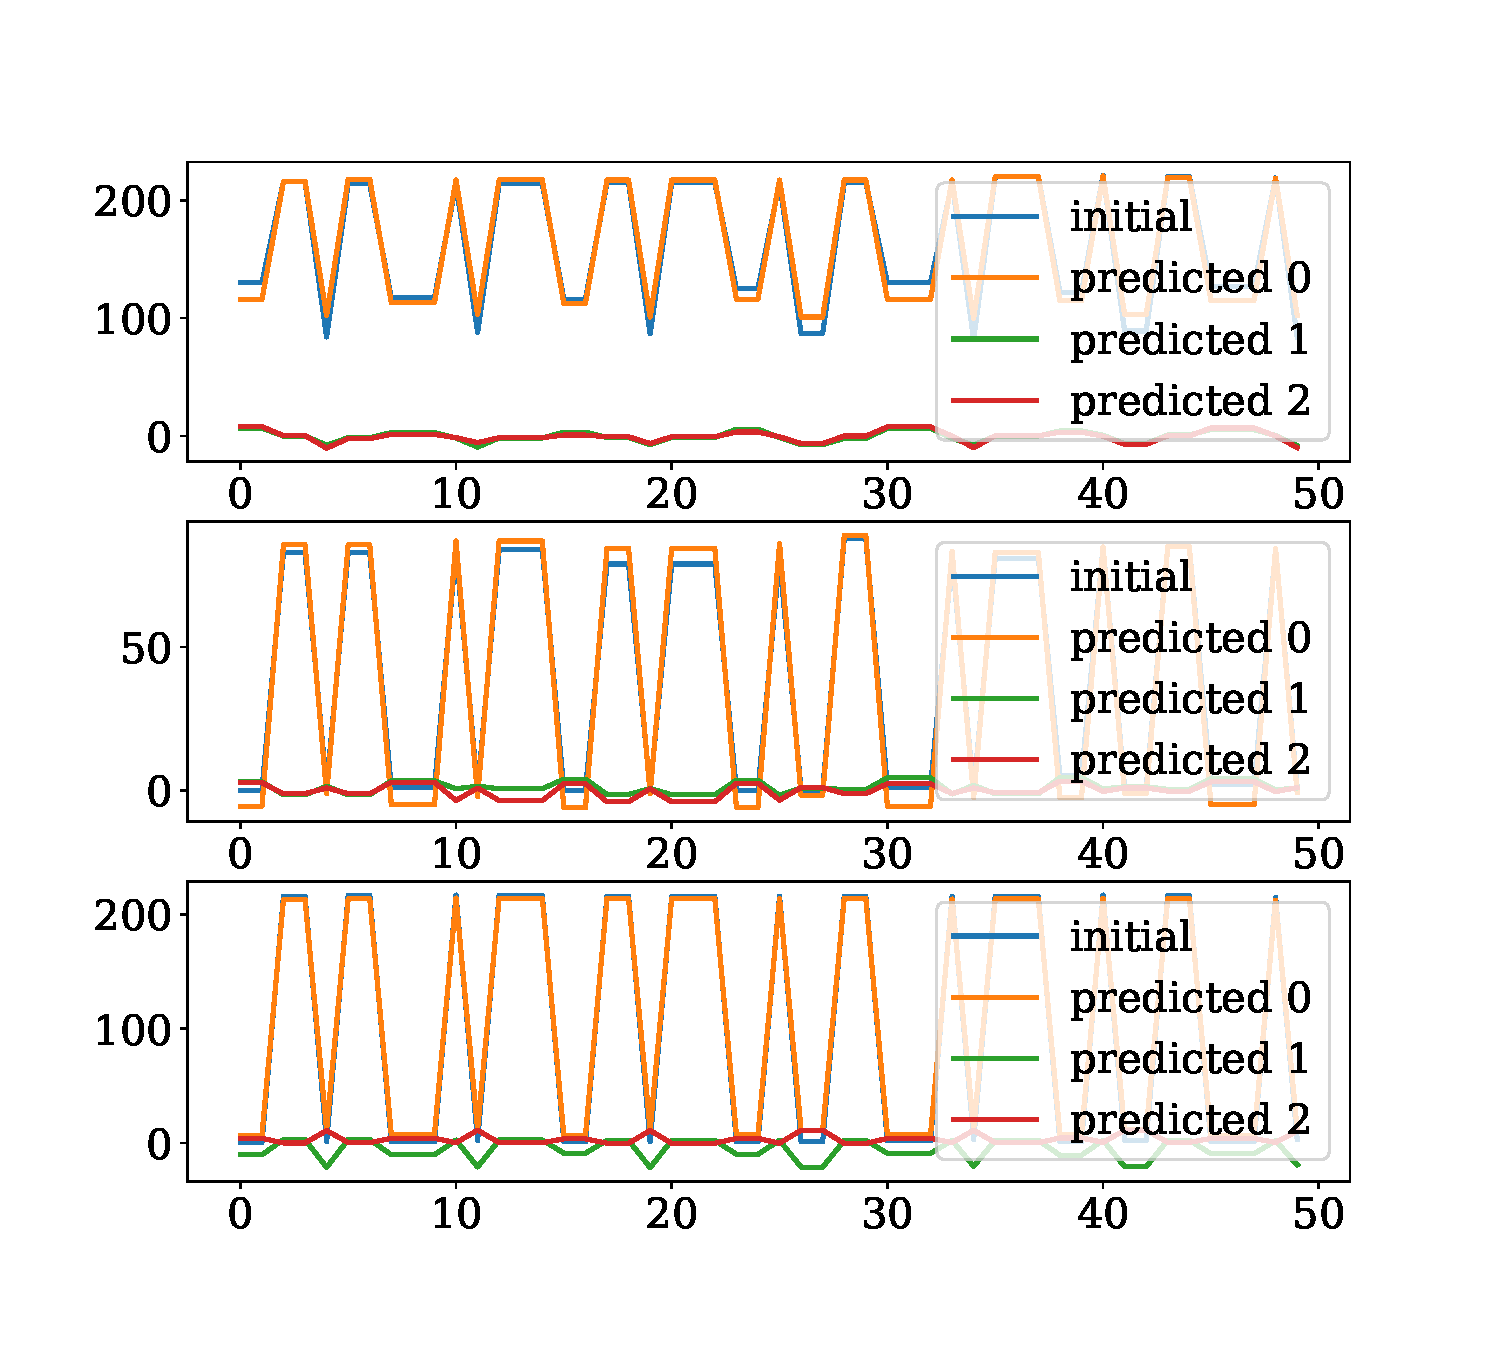
\includegraphics[width=0.6\textwidth]{sections/gorpinich/ssa_mario.pdf}
\caption{Some description}
\label{fig:4}
\end{figure}

Fig. \ref{fig:4} plots SSA decomposition of the more complex video.

\end{document}